% Provenance (never printed): old terminale S material on the continental crust
% (granitic composition, thickness, density, age; roots and isostasy). Thickness
% from Christensen-Mooney 1995 and Cogley 1984 (CRUST1.0 dropped: no licence,
% Sync 1); ocean-floor ages from figdata/grade-12/crust_ages.py (Seton 2020 grid,
% as in g11.01). Airy isostasy is g11.03's: recalled, not re-derived. Radiometric
% dating is g12.07's: ages are only quoted here.
\chapter{महाद्वीपीय भूपर्पटी}\label{ch:g12:continental-crust}

उत्तर-पश्चिमी कनाडा में, अकास्टा नदी के पास, हल्की और गहरी पट्टियों से धारीदार
एक धूसर चट्टान सतह पर दिखती है। उसकी आयु 4.00 से 4.03 अरब
वर्ष आँकी गई है: अकास्टा नाइस, ज्ञात सबसे पुरानी चट्टान। उससे भी पुराने हैं
खनिज ज़र्कॉन के कण, हर एक मिलीमीटर का एक अंश लंबा, जो पश्चिमी ऑस्ट्रेलिया की
जैक हिल्स की पुरानी अवसादी चट्टानों में मिले। और भी पुरानी
चट्टानों से घिसकर निकले और दबने से पहले पानी द्वारा बहाए गए ये कण 4.4
अरब वर्ष पहले क्रिस्टलित हुए थे, और दिखाते हैं कि तब एक भूपर्पटी मौजूद थी। कोई भी महासागरीय तली इसकी बीसवें भाग जितनी भी पुरानी नहीं। यह अध्याय
पूछता है कि महाद्वीप किससे बने हैं, और वे टिके क्यों रहते हैं।
% ledger: bowring99:acasta, wilde01:zircon, uw14:jack-hills, photo:g12-acasta, photo:g12-jack-hills-zircons

\begin{omfigure}
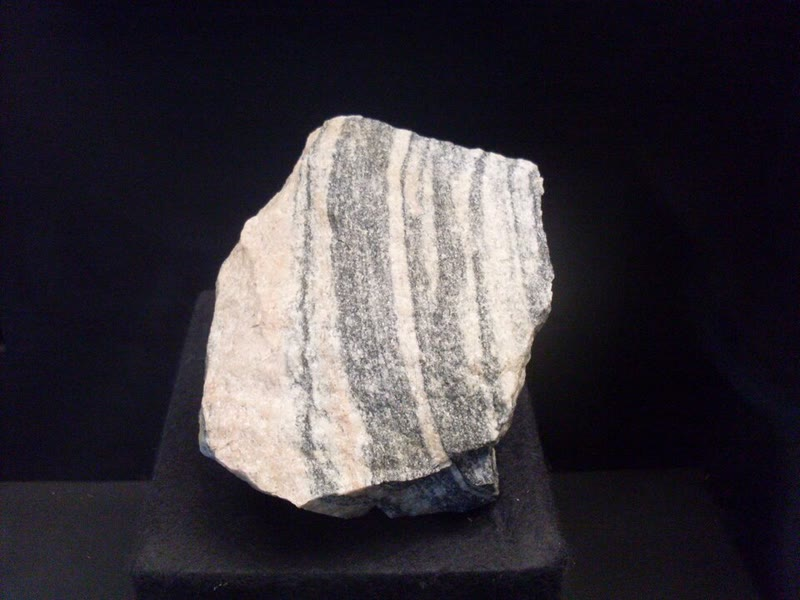
\includegraphics[height=4.6cm]{images/book2/g12-pedro-acasta-gneiss.jpg}\hspace{0.04\linewidth}%
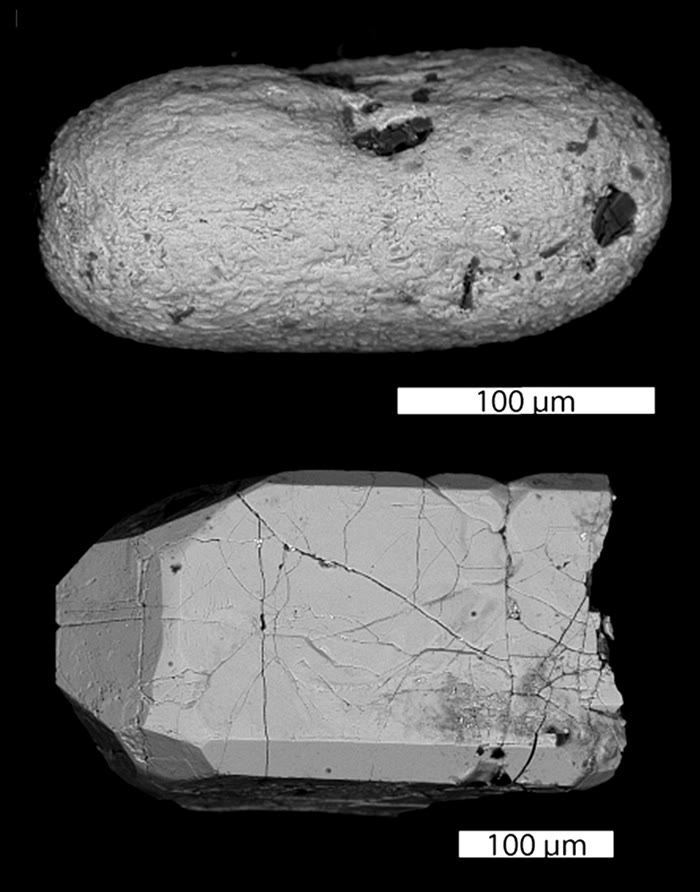
\includegraphics[height=4.6cm]{images/book2/g12-cavosie-jack-hills-zircons.jpg}

{\small बाएँ: अकास्टा नाइस का एक टुकड़ा, 4.03 अरब वर्ष पुराना, एक
संग्रहालय-प्रदर्शनी में। फ़ोटो पेद्रोअलेक्ज़ांद्रादे (CC~BY-SA~3.0)। दाएँ: पश्चिमी ऑस्ट्रेलिया की
जैक हिल्स के ज़र्कॉन के दो कण, इलेक्ट्रॉन
सूक्ष्मदर्शी से देखे गए; हर पैमाना-पट्टी \qty{100}{\micro m} की है। ऊपर का कण
पानी द्वारा बहाए जाते समय गोल हो गया, नीचे वाले ने अपने क्रिस्टल-फलक बनाए रखे।
चित्र ए॰~कैवोसी और जे॰~वैली (सार्वजनिक डोमेन)।}
\end{omfigure}
% ledger: photo:g12-acasta, photo:g12-jack-hills-zircons

\begin{recall}
भूपर्पटी \omterm{def:g11:seismic-structure:moho}{मोहो} पर समाप्त होती है, जिसके नीचे अधिक घना प्रावार है
(\cref{ch:g11:seismic-structure})। \omterm{def:g11:ocean-ridges:oceanic-lithosphere}{महासागरीय भूपर्पटी} कटकों पर बनी लगभग \qty{7}{km}
बेसाल्ट और \omterm{def:g11:ocean-ridges:gabbro}{गैब्रो} है (\cref{ch:g11:ocean-ridges}), और वह
कभी लगभग 190 मिलियन वर्ष से अधिक पुरानी नहीं होती (\cref{ch:g11:drift-to-spreading})।
बाहरी परतें \omterm{def:g11:lithosphere-asthenosphere:lithosphere}{दुर्बलतामंडल} पर तैरती हैं: एयरी के मॉडल में, जो क्षेत्र
ऊँचाई $h$ अधिक ऊँचा खड़ा है, उसकी भूपर्पटी $h\,\rho_m/(\rho_m -
\rho_c)$ अधिक मोटी होती है (\cref{ch:g11:lithosphere-asthenosphere})। आग्नेय चट्टानों के नाम
उनके \omterm{def:g11:igneous-rocks:texture}{गठन} और उनकी सिलिका-मात्रा से रखे जाते हैं: \omterm{def:g11:igneous-rocks:felsic-mafic}{मैफ़िक} 45 से
\qty{55}{\percent} \ce{SiO2}, \omterm{def:g11:igneous-rocks:felsic-mafic}{मध्यवर्ती} 55 से 65, \omterm{def:g11:igneous-rocks:felsic-mafic}{फ़ेल्सिक} 65 से
75 (\cref{ch:g11:igneous-rocks})। रेडियोधर्मी तत्त्व स्थिर दर से क्षयित होते
हैं, जिससे चट्टानों को उनकी आयु मिलती है (भौतिकी की पुस्तकें;
\cref{ch:g12:age-of-the-earth})।
\end{recall}
% ledger: white92:crust, data:b2-seafloor-age, tulane:magma-types

\section{महाद्वीप किससे बने हैं}

\begin{definition}[महाद्वीपीय भूपर्पटी]\label{def:g12:continental-crust:continental-crust}
\emph{महाद्वीपीय भूपर्पटी}\index{महाद्वीपीय भूपर्पटी} वह भूपर्पटी है जो
महाद्वीपों को बनाती है, उनके उथले समुद्रों के नीचे के भागों सहित। यह
मोटी है, अपने ऊपरी भाग में औसतन ग्रेनाइटी संघटन की, हल्की, और यह
बहुत पुरानी हो सकती है।
\end{definition}
% ledger: tulane:crust-types, tulane:roots, cogley84:continents

महाद्वीप स्थल से बड़े हैं। \omterm{def:g12:continental-crust:continental-crust}{महाद्वीपीय भूपर्पटी} के किनारे
समुद्र के नीचे, महाद्वीपीय मग्नतटों पर, हैं: इस तरह मानचित्रित करने पर
\omterm{def:g12:continental-crust:continental-crust}{महाद्वीपीय भूपर्पटी} \num{210}~मिलियन~\unit{km^2} ढकती है, पृथ्वी की सतह का
\qty{41}{\percent}, जिसका लगभग एक-तिहाई, \qty{30.6}{\percent},
जलमग्न है। अपने जलमग्न भागों सहित गिनने पर
\omterm{def:g12:continental-crust:continental-crust}{महाद्वीपीय भूपर्पटी} की माध्य ऊँचाई समुद्र-तल से केवल लगभग \qty{120}{m} है।
% ledger: cogley84:continents

सतह पर महाद्वीप हर प्रकार की चट्टान दिखाते हैं --- अवसाद,
\omterm{def:g11:igneous-rocks:volcanic-plutonic}{ज्वालामुखीय चट्टानें}, कायांतरित चट्टानें --- पर अवसादी आवरण के नीचे
\omterm{def:g12:continental-crust:continental-crust}{महाद्वीपीय भूपर्पटी} ज़्यादातर ग्रेनाइटी चट्टानों से और पुराने पर्वत-मूलों की कायांतरित
और \omterm{def:g11:igneous-rocks:volcanic-plutonic}{पातालीय चट्टानों} से बनी है। औसतन समग्र \omterm{def:g12:continental-crust:continental-crust}{महाद्वीपीय
भूपर्पटी} में \qty{60.6}{\percent} सिलिका है; उसका ऊपरी भाग अधिक समृद्ध है,
\qty{66.6}{\percent}, इसलिए उसका गहरा भाग अधिक निर्धन होना चाहिए।
% ledger: rg14:crust, tulane:crust-types, cm95:crust

\begin{omfigure}
\begin{tikzpicture}
\begin{axis}[omrecord, ybar=0pt, width=0.92\linewidth, height=5.0cm, bar width=7pt,
  ymin=0, ymax=80, ylabel={द्रव्यमान-अंश (\unit{\percent})},
  symbolic x coords={SiO2, Al2O3, FeO, MgO, CaO, Na2O, K2O},
  xticklabels={\ce{SiO2}, \ce{Al2O3}, \ce{FeO}, \ce{MgO}, \ce{CaO}, \ce{Na2O}, \ce{K2O}},
  xtick=data, enlarge x limits=0.08, ymajorgrids=true, xmajorgrids=false,
  legend style={font=\scriptsize, at={(0.98,0.97)}, anchor=north east, legend columns=1}]
% ledger: rg14:crust (upper and bulk continental crust; FeO* total iron)
\addplot[fill=omLithGranite, draw=black!60] coordinates {(SiO2,66.6) (Al2O3,15.4) (FeO,5.04) (MgO,2.48) (CaO,3.59) (Na2O,3.27) (K2O,2.80)};
\addplot[fill=omProp!55, draw=black!60] coordinates {(SiO2,60.6) (Al2O3,15.9) (FeO,6.71) (MgO,4.66) (CaO,6.41) (Na2O,3.07) (K2O,1.81)};
% ledger: earle:magma-oxides (mafic magma: midpoint of each range, the bar spans the range)
\addplot[fill=omLithBasalt, draw=black!60, error bars/.cd, y dir=both, y explicit]
  coordinates {(SiO2,50) +- (0,5) (Al2O3,16) +- (0,2) (FeO,10) +- (0,2) (MgO,7) +- (0,2) (CaO,9) +- (0,2) (Na2O,2) +- (0,1) (K2O,1.75) +- (0,1.25)};
\legend{ऊपरी महाद्वीपीय भूपर्पटी, समग्र महाद्वीपीय भूपर्पटी, मैफ़िक मैग्मा (परास)}
\end{axis}
\end{tikzpicture}

{\small \omterm{def:g11:igneous-rocks:felsic-mafic}{मैफ़िक} मैग्मा से तुलना में \omterm{def:g12:continental-crust:continental-crust}{महाद्वीपीय भूपर्पटी} का संघटन, वह
मैग्मा जो \omterm{def:g11:ocean-ridges:oceanic-lithosphere}{महासागरीय भूपर्पटी} बनाता है: मुख्य ऑक्साइड, द्रव्यमान के प्रतिशत में
(\ce{FeO} सारा लोहा गिनता है)। \omterm{def:g12:continental-crust:continental-crust}{महाद्वीपीय भूपर्पटी} सिलिका,
सोडियम और पोटैशियम से अधिक समृद्ध है, लोहे, मैग्नीशियम और कैल्सियम में अधिक निर्धन। आँकड़े: रुडनिक
और गाओ (2014); \omterm{def:g11:igneous-rocks:felsic-mafic}{मैफ़िक} परास एस॰~अर्ल, \emph{भौतिक भूविज्ञान}
(CC~BY~4.0) से।}
\end{omfigure}
% ledger: rg14:crust, earle:magma-oxides

\section{एक मोटी, हल्की भूपर्पटी}

भूकंपीय सर्वेक्षण महाद्वीपों के नीचे \omterm{def:g11:seismic-structure:moho}{मोहो} को बहुत भिन्न
गहराइयों पर पाते हैं। सभी महाद्वीपों पर, क्षेत्रफल से भारित, औसत लेने पर भूपर्पटी लगभग
\qty{41}{km} मोटी है; जहाँ भूपर्पटी खिंची है वहाँ वह पतली है, लगभग \qty{30}{km},
और पर्वत-पट्टियों में मोटी, औसतन लगभग \qty{46}{km}।
पर्वत-पट्टियों से दूर वह सामान्यतः 35 से \qty{40}{km} मोटी है;
सबसे ऊँची श्रेणियों के नीचे 50 से \qty{70}{km}, तिब्बत के कुछ भागों के नीचे लगभग \qty{70}{km}।
\omterm{def:g11:ocean-ridges:oceanic-lithosphere}{महासागरीय भूपर्पटी} लगभग \qty{7}{km} मोटी है: \omterm{def:g12:continental-crust:continental-crust}{महाद्वीपीय भूपर्पटी} पाँच
से दस गुना अधिक मोटी है।
% ledger: cm95:crust, tulane:roots, karplus:tibet-moho, white92:crust

\begin{omfigure}
\begin{tikzpicture}
\begin{axis}[omrecord, xbar, bar shift=0pt, width=0.78\linewidth, height=5.0cm, bar width=8pt,
  xmin=0, xmax=80, ymin=0.4, ymax=5.6, ytick={1,...,5},
  yticklabels={महासागरीय भूपर्पटी, खिंचे महाद्वीप, महाद्वीप (औसत), पर्वत-पट्टियाँ (औसत), तिब्बत के नीचे},
  xlabel={भूपर्पटी की मोटाई (\unit{km})}, ymajorgrids=false,
  nodes near coords, nodes near coords style={font=\scriptsize, anchor=west}, point meta=explicit symbolic]
% ledger: white92:crust, cm95:crust, karplus:tibet-moho
\addplot[fill=omLithBasalt, draw=black!60] coordinates {(7.1,1) [7.1]};
\addplot[fill=omLithGranite, draw=black!60] coordinates {(30.5,2) [30.5] (41.1,3) [41.1] (46.3,4) [46.3] (70,5) [लगभग 70]};
\end{axis}
\end{tikzpicture}

{\small भूकंपीय मापनों से भूपर्पटी की मोटाई। आँकड़े: \omterm{def:g11:ocean-ridges:oceanic-lithosphere}{महासागरीय भूपर्पटी} के लिए व्हाइट,
मैकेंज़ी और ओ'नायंस (1992); महाद्वीपीय औसतों के लिए क्रिस्टेनसेन और मूनी
(1995); तिब्बत के लिए कार्पलस और अन्य (2019)।}
\end{omfigure}
% ledger: white92:crust, cm95:crust, karplus:tibet-moho

\omterm{def:g12:continental-crust:continental-crust}{महाद्वीपीय भूपर्पटी} हल्की भी है। उसका माध्य घनत्व लगभग
\qty{2830}{kg/m^3} है। \omterm{def:g11:ocean-ridges:oceanic-lithosphere}{महासागरीय भूपर्पटी} के बेसाल्ट और \omterm{def:g11:ocean-ridges:gabbro}{गैब्रो},
पाइरॉक्सीन और ओलिवीन से समृद्ध, लगभग \qty{3000}{kg/m^3} तक आते हैं
(\cref{ch:g11:minerals}), और \omterm{def:g11:seismic-structure:moho}{मोहो} के ठीक नीचे का प्रावार लगभग
\qty{3380}{kg/m^3} तक। मोटी और हल्की भूपर्पटी ऊँची तैरती है: यही कारण है कि
महाद्वीप महासागरीय तली से ऊपर खड़े हैं, और कोई महाद्वीप किसी \omterm{def:g11:subduction-zones:subduction}{क्षेपण
क्षेत्र} पर नीचे क्यों नहीं घसीटा जा सकता। जहाँ कोई महाद्वीप किसी खाई तक पहुँचता है, वह डूबने के लिए
बहुत हल्का होता है; \omterm{def:g11:subduction-zones:subduction}{क्षेपण} रुक जाता है, और दोनों महाद्वीप टकराते हैं
(\cref{ch:g12:mountain-building})। \omterm{def:g12:continental-crust:continental-crust}{महाद्वीपीय भूपर्पटी}, एक बार बन जाने पर, नष्ट करना
कठिन है।
% ledger: cm95:crust, data:prem, tulane:roots, tulane:no-subduct
% values (mineral_density.py): basalt/gabbro rock line 3.0015 g/cm3

\begin{omfigure}
\begin{tikzpicture}[x=1cm, y=0.075cm, font=\footnotesize]
  % continental column: 41 km of crust, surface at +0.12 km (mean height); ocean column: 3.7 km of water drawn schematically
  \fill[omLithGranite] (0,0) rectangle (3,-41);
  \fill[omLithPeridotite!60] (0,-41) rectangle (3,-60);
  \fill[omSea] (6,0) rectangle (9,-4);
  \fill[omLithGabbro] (6,-4) rectangle (9,-11.1);
  \fill[omLithPeridotite!60] (6,-11.1) rectangle (9,-60);
  \draw[black!60] (0,0) rectangle (3,-60) (6,0) rectangle (9,-60);
  \draw[line width=0.9pt] (0,-41) -- (3,-41) (6,-11.1) -- (9,-11.1);
  \node[align=center] at (1.5,-20) {महाद्वीपीय भूपर्पटी\\लगभग \qty{41}{km}\\\qty{2830}{kg/m^3}\\4 अरब वर्ष तक};
  \node[align=center] at (7.5,-24) {प्रावार\\\qty{3380}{kg/m^3}\\मोहो के नीचे};
  \node[align=center] at (1.5,-50.5) {प्रावार};
  \node at (7.5,-2) {महासागर};
  \draw[black!60] (8.6,-7.6) -- (9.3,-7.6);
  \node[anchor=west, align=left] at (9.3,-7.6) {महासागरीय भूपर्पटी, लगभग \qty{7}{km}\\\qty{3000}{kg/m^3}\\200 मिलियन वर्ष से कम};
  \node[anchor=east] at (-0.1,-41) {मोहो};
  \node[anchor=east] at (5.9,-11.1) {मोहो};
  \node[anchor=south] at (1.5,0) {एक महाद्वीप};
  \node[anchor=south] at (7.5,0) {एक महासागर};
  \foreach \d in {0,20,40,60} {\draw[black!60] (-1.5,-\d) -- (-1.3,-\d); \node[anchor=east, font=\scriptsize] at (-1.5,-\d) {\d};}
  \draw[black!60] (-1.4,0) -- (-1.4,-60);
  \node[rotate=90, font=\scriptsize] at (-2.3,-30) {गहराई (\unit{km})};
\end{tikzpicture}

{\small अगल-बगल एक महाद्वीप और एक महासागर (गहराइयाँ पैमाने पर, चौड़ाइयाँ नहीं;
महासागर \qty{4}{km} गहरा खींचा गया): \omterm{def:g12:continental-crust:continental-crust}{महाद्वीपीय भूपर्पटी} \omterm{def:g11:ocean-ridges:oceanic-lithosphere}{महासागरीय भूपर्पटी} से अधिक मोटी, हल्की
और कहीं अधिक पुरानी है।}
\end{omfigure}
% ledger: cm95:crust, white92:crust, data:prem, bowring99:acasta, data:b2-seafloor-age

\begin{method}[महाद्वीपीय और महासागरीय भूपर्पटी की तुलना]\label{met:g12:continental-crust:compare}
किसी स्थान के नीचे किस प्रकार की भूपर्पटी है, यह बताने के लिए पाँच गुणों की तुलना कीजिए:
\begin{enumerate}
  \item मोटाई: \omterm{def:g11:ocean-ridges:oceanic-lithosphere}{महासागरीय भूपर्पटी} के लिए लगभग \qty{7}{km}, \omterm{def:g12:continental-crust:continental-crust}{महाद्वीपीय भूपर्पटी} के लिए 30 से
        \qty{70}{km};
  \item चट्टानें: बेसाल्ट और \omterm{def:g11:ocean-ridges:gabbro}{गैब्रो}, या अवसादों के आवरण के नीचे ग्रेनाइट, नाइस और उनकी
        संबंधी चट्टानें;
  \item संघटन: लगभग \qty{50}{\percent} सिलिका, या लगभग 60 और
        अधिक;
  \item घनत्व: लगभग \qty{3000}{kg/m^3}, या लगभग \qty{2830}{kg/m^3};
  \item आयु: 200 मिलियन वर्ष से कम, या 4 अरब वर्ष तक।
\end{enumerate}
ऊँचाई एक सुराग है, परीक्षण नहीं: महासागरीय तली का अधिकांश भाग
किलोमीटरों गहरा है, पर महाद्वीपों के किनारे उथले समुद्रों के नीचे हैं।
\end{method}
% ledger: white92:crust, cm95:crust, rg14:crust, earle:magma-oxides, cogley84:continents

\begin{example}[एक उथली समुद्री तली]\label{ex:g12:continental-crust:shelf}
एक सर्वेक्षण-पोत \qty{150}{m} गहरी समुद्री तली पाता है। भूकंपीय प्रोफ़ाइलें
\omterm{def:g11:seismic-structure:moho}{मोहो} को समुद्री तली से \qty{32}{km} नीचे रखती हैं; एक वेध-कोर
अवसादों के नीचे से क्वार्ट्ज़, फ़ेल्डस्पार और अभ्रक की एक स्थूलकणी चट्टान ऊपर लाता है। वहाँ कौन-सी भूपर्पटी
है?

\emph{हल।} मोटाई लगभग \qty{32}{km}: महाद्वीपीय, औसत से
पतली, जैसी वहाँ होती है जहाँ वह खिंची हो। अवसादों के नीचे ग्रेनाइट:
महाद्वीपीय। यह समुद्री तली एक महाद्वीपीय मग्नतट है, उन जलमग्न
भागों में से एक जो महाद्वीपों का लगभग एक-तिहाई बनाते हैं।
\end{example}
% invented numbers; ledger: cm95:crust, cogley84:continents

यह सारी भूपर्पटी कितनी भारी है? पृथ्वी की त्रिज्या की तुलना में पतली परत का
द्रव्यमान सरल होता है।

\begin{proposition}[पतली परत का द्रव्यमान]\label{prop:g12:continental-crust:thin-layer}
मोटाई $H$ और घनत्व $\rho$ की कोई परत किसी ग्रह की सतह का अंश $f$ ढकती है;
ग्रह की त्रिज्या $R \gg H$ है और माध्य घनत्व $\bar\rho$। तब परत का
द्रव्यमान $m \approx 4\pi R^2 f H \rho$ है, और ग्रह के द्रव्यमान $M$ में उसका भाग यह है:
\[
  \frac{m}{M} \approx 3 f\,\frac{H}{R}\,\frac{\rho}{\bar\rho}.
\]
\end{proposition}
% ledger: earth:Rmean, earth:density

\begin{proof}
ग्रह की सतह $4\pi R^2$ है; परत $4\pi R^2 f$ ढकती है और,
पतली होने के कारण, उसका आयतन उस क्षेत्रफल गुणा $H$ के निकट है, इसलिए $m \approx 4\pi R^2
f H \rho$। ग्रह का द्रव्यमान $M = \tfrac{4}{3}\pi R^3 \bar\rho$ है। भाग देने पर,
$m/M \approx 4\pi R^2 f H \rho / (\tfrac{4}{3}\pi R^3 \bar\rho) = 3 f (H/R)
(\rho/\bar\rho)$।
\end{proof}

\omterm{def:g11:ocean-ridges:oceanic-lithosphere}{महासागरीय भूपर्पटी} के लिए --- सतह का शेष \qty{59}{\percent},
\qty{7.1}{km}, लगभग \qty{3000}{kg/m^3} --- $R = \qty{6371}{km}$ और
$\bar\rho = \qty{5513}{kg/m^3}$ के साथ, भाग $3 \times 0.59 \times
(7.1/6371) \times (3000/5513) \approx 0.0011$ है: पृथ्वी के द्रव्यमान के
एक प्रतिशत का लगभग दसवाँ भाग। सप्ताहांत समस्या महाद्वीपों के लिए यही करती है।
% ledger: cogley84:continents, white92:crust, earth:Rmean, earth:density

\section{एक पुरानी भूपर्पटी}

महासागरीय तली हर जगह नई है: उसका तीन-चौथाई भाग 100 मिलियन वर्ष से
नया है, और लगभग कुछ भी 190 मिलियन वर्ष से पुराना नहीं। महाद्वीपों की
बात अलग है। उनकी चट्टानें पृथ्वी के लगभग पूरे इतिहास में फैली हैं,
4.03 अरब वर्ष पुराने अकास्टा नाइस से लेकर आज फूटे
लावाओं तक, और ज़र्कॉन के कण अभिलेख को 4.4 अरब वर्ष पीछे तक ले जाते हैं।
% ledger: data:b2-seafloor-age, bowring99:acasta, uw14:jack-hills

\begin{omfigure}
\begin{tikzpicture}
\begin{axis}[omrecord, ybar interval, width=0.82\linewidth, height=5.0cm,
  xmin=0, xmax=200, ymin=0, ymax=0.12, xtick={0,20,...,200},
  xlabel={महासागरीय तली की आयु (मिलियन वर्ष)},
  ylabel={महासागरीय तली का भाग}, yticklabel style={/pgf/number format/fixed},
  ymajorgrids=true, xmajorgrids=false, clip=false, x tick label as interval=false]
% computed in figdata/grade-12/crust_ages.py (Seton 2020 grid, 1-degree cells, area-weighted)
\addplot[fill=omDef!35, draw=omDef] table[x=age_lo, y=share] {figdata/out/grade-12-crust_ages-hist.dat};
\node[anchor=north east, align=right, font=\scriptsize, fill=white, inner sep=2pt] at (axis cs:198,0.115)
  {सबसे पुरानी महाद्वीपीय चट्टान: \num{4030} मिलियन वर्ष,\\सबसे पुरानी महासागरीय तली से बीस गुना पुरानी};
\end{axis}
\end{tikzpicture}

{\small महासागरीय तली कितनी पुरानी है: 10
मिलियन वर्ष की हर पट्टी में उसके क्षेत्रफल का भाग। नई तली प्रधान है; 190
मिलियन वर्ष से पुराना लगभग कुछ भी नहीं (पूर्वी भूमध्यसागर की कुछ पुरानी द्रोणियाँ छोड़ दी गई हैं)।
आँकड़े: सेटन और अन्य (2020), परिकलित।}
\end{omfigure}
% ledger: data:b2-seafloor-age, bowring99:acasta
% values (crust_ages.py): oldest_open_myr 192.5, share_younger_100 0.765, share_younger_150 0.956, rock_over_floor 20.9

महाद्वीपों के सबसे पुराने भाग उनके क्रोड बनाते हैं।

\begin{definition}[क्रेटन]\label{def:g12:continental-crust:craton}
\emph{क्रेटन}\index{क्रेटन} किसी महाद्वीप का एक पुराना और स्थिर क्रोड है:
एक अरब वर्ष से भी पहले बनी और विकृत हुई \omterm{def:g12:continental-crust:continental-crust}{महाद्वीपीय भूपर्पटी}, जो
तब से ठंडी हो चुकी है और अब विकृत नहीं होती। उसकी चट्टानें ज़्यादातर कायांतरित और
\omterm{def:g11:igneous-rocks:volcanic-plutonic}{पातालीय चट्टानें} हैं, पूर्व पर्वतों के गहरे \omterm{def:g12:continental-crust:root}{मूल}।
\end{definition}
% ledger: tulane:cratons

\omterm{def:g12:continental-crust:craton}{क्रेटनों} के चारों ओर नई विकृत चट्टानों की पट्टियाँ हैं, बाद में बनी
पर्वत-श्रेणियों के अपरदित \omterm{def:g12:continental-crust:root}{मूल}; पट्टियाँ किसी महाद्वीप के किनारों की ओर नई होती
जाती हैं। कोई महाद्वीप पर्वत-निर्माण से बढ़ा है जिसने एक प्राचीन क्रोड के चारों ओर
उसके किनारों पर नई भूपर्पटी जोड़ी। कनाडा में, जहाँ \omterm{def:g12:continental-crust:craton}{क्रेटन} की
चट्टानें सतह पर हैं, 1 से 3 अरब वर्ष पुराने नाइस और ग्रेनाइट
दिखते हैं, जैसे यहाँ एक झील-तट पर।
% ledger: tulane:cratons, photo:g12-canadian-shield

\begin{omfigure}
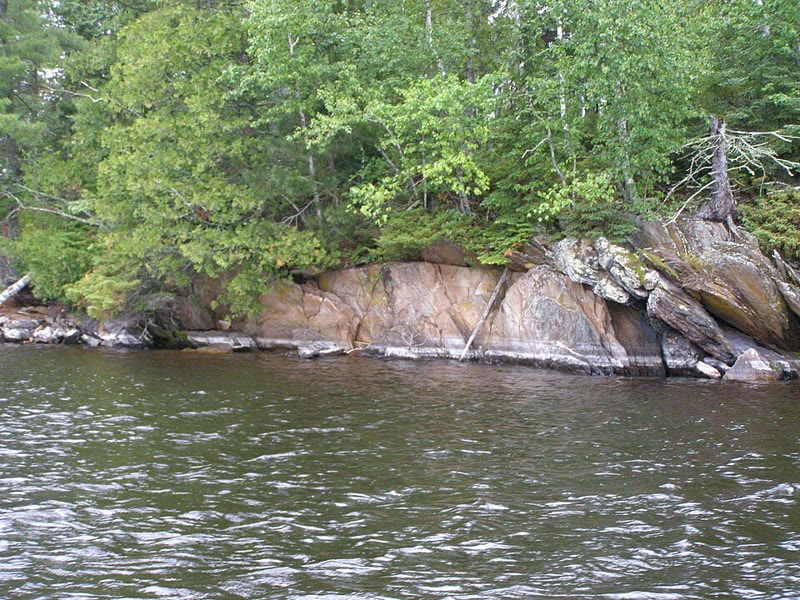
\includegraphics[height=5.0cm]{images/book2/g12-light-canadian-shield.jpg}

{\small कनाडा में एक झील-तट पर 1 से 3 अरब वर्ष पुराने नाइस और ग्रेनाइट,
उत्तरी अमेरिका के प्राचीन क्रोड का भाग। फ़ोटो क्रिस लाइट
(CC~BY-SA~4.0)।}
\end{omfigure}
% ledger: photo:g12-canadian-shield

\omterm{def:g12:continental-crust:continental-crust}{महाद्वीपीय भूपर्पटी} क्यों टिकी रहती है, जबकि महासागरीय तली हमेशा नई होती है?
\omterm{def:g11:ocean-ridges:oceanic-lithosphere}{महासागरीय भूपर्पटी} घनी है: वह \omterm{def:g11:subduction-zones:subduction}{क्षेपण क्षेत्रों} पर वापस प्रावार में डूब जाती है,
और उसका कोई भी भाग 200 मिलियन वर्ष से बहुत अधिक नहीं बचता। \omterm{def:g12:continental-crust:continental-crust}{महाद्वीपीय
भूपर्पटी} डूबने के लिए बहुत हल्की है; उसे अपरदन घिस सकता है, खींच सकता है या
सिकोड़ सकता है, पर वह सतह पर बनी रहती है। किसी महाद्वीप की चट्टानें
चार अरब वर्षों का अभिलेखागार हैं।
% ledger: tulane:no-subduct, tulane:roots, data:b2-seafloor-age

\section{पर्वत-मूल}

पर्वत जितने ऊँचे, उनके नीचे की भूपर्पटी उतनी ही मोटी।

\begin{definition}[पर्वत-मूल]\label{def:g12:continental-crust:root}
किसी पर्वत-श्रेणी का \emph{मूल}\index{मूल (पर्वत-श्रेणी का)} उसकी
मोटी हुई भूपर्पटी का वह भाग है जो आसपास की निचली भूमियों के नीचे के \omterm{def:g11:seismic-structure:moho}{मोहो} के
स्तर से नीचे प्रावार में पहुँचता है।
\end{definition}
% ledger: tulane:roots

एयरी का मॉडल \omterm{def:g12:continental-crust:root}{मूल} की भविष्यवाणी करता है: अपने परिवेश से $h$ ऊपर खड़ी
श्रेणी का \omterm{def:g12:continental-crust:root}{मूल} $r = h\,\rho_c/(\rho_m - \rho_c)$ होता है, $\rho_c = \qty{2830}{kg/m^3}$ और $\rho_m =
\qty{3380}{kg/m^3}$ के साथ उसकी ऊँचाई का लगभग पाँच गुना
(\cref{prop:g11:lithosphere-asthenosphere:airy})। दो
प्रकार के मापन \omterm{def:g12:continental-crust:root}{मूलों} को देखते हैं। भूकंपीय सर्वेक्षण श्रेणियों के नीचे \omterm{def:g11:seismic-structure:moho}{मोहो} को अधिक
गहरा पाते हैं: बहुत-सी पर्वत-पट्टियों के नीचे 50 से \qty{70}{km}, तिब्बत के कुछ भागों के नीचे लगभग
\qty{70}{km}। पर्वत-श्रेणियों के ऊपर गुरुत्व उससे कमज़ोर होता है जितना
उनका दृश्य द्रव्यमान सुझाता: हल्का \omterm{def:g12:continental-crust:root}{मूल}, अधिक घने प्रावार के स्थान पर खड़ा,
गहराई पर द्रव्यमान की कमी बनाता है, और मापी गई गुरुत्व
विसंगतियाँ स्थलाकृति और भूकंपविज्ञान द्वारा पाई गई भूपर्पटी की मोटाई का
अनुसरण करती हैं। महाद्वीप तैरते हैं, और उनके पर्वत सबसे ऊँचे तैरते हैं।
% ledger: tulane:roots, karplus:tibet-moho, cm95:crust, data:prem

\section{अभ्यास}

\begin{exercise}[$\star$]\label{exo:g12:continental-crust:1}
महाद्वीपीय और \omterm{def:g11:ocean-ridges:oceanic-lithosphere}{महासागरीय भूपर्पटी} के लिए उतारकर पूरा कीजिए: मोटाई;
मुख्य चट्टानें; सिलिका-मात्रा; घनत्व; अधिकतम आयु।
\end{exercise}

\begin{exercise}[$\star$]\label{exo:g12:continental-crust:2}
समग्र \omterm{def:g12:continental-crust:continental-crust}{महाद्वीपीय भूपर्पटी} में \qty{60.6}{\percent} सिलिका है, उसके ऊपरी
भाग में \qty{66.6}{\percent}। आग्नेय चट्टानों के सिलिका-वर्गों का उपयोग करके बताइए कि
हर एक \omterm{def:g11:igneous-rocks:felsic-mafic}{मैफ़िक}, \omterm{def:g11:igneous-rocks:felsic-mafic}{मध्यवर्ती} या \omterm{def:g11:igneous-rocks:felsic-mafic}{फ़ेल्सिक} है? उसी संघटन की एक \omterm{def:g11:igneous-rocks:volcanic-plutonic}{पातालीय चट्टान} का
नाम बताइए।
\end{exercise}

\begin{exercise}[$\star$]\label{exo:g12:continental-crust:3}
\omterm{def:g11:ocean-ridges:oceanic-lithosphere}{महासागरीय भूपर्पटी} किसी \omterm{def:g11:subduction-zones:subduction}{क्षेपण क्षेत्र} पर प्रावार में क्यों डूब सकती है, और
\omterm{def:g12:continental-crust:continental-crust}{महाद्वीपीय भूपर्पटी} क्यों नहीं? घनत्वों से उत्तर दीजिए।
\end{exercise}

\begin{exercise}[$\star$]\label{exo:g12:continental-crust:4}
(1) \omterm{def:g12:continental-crust:craton}{क्रेटन} क्या है? (2) \omterm{def:g12:continental-crust:craton}{क्रेटन} की चट्टानें कम से कम कितनी पुरानी होती हैं?
(3) कौन-से प्रकार की चट्टानें इसे बनाती हैं?
\end{exercise}

\begin{exercise}[$\star$]\label{exo:g12:continental-crust:5}
सबसे पुरानी महासागरीय तली लगभग 190 मिलियन वर्ष पुरानी है, अकास्टा नाइस
4.03 अरब वर्ष। नाइस कितने गुना अधिक पुराना है? उतनी पुरानी कोई महासागरीय तली
क्यों नहीं है?
\end{exercise}

\begin{exercise}[$\star\star$]\label{exo:g12:continental-crust:6}
\omterm{def:g12:continental-crust:continental-crust}{महाद्वीपीय भूपर्पटी} \num{210.4}~मिलियन~\unit{km^2} ढकती है, जिसका
\qty{30.6}{\percent} समुद्र के नीचे है। (1) \omterm{def:g12:continental-crust:continental-crust}{महाद्वीपीय भूपर्पटी} का कितना क्षेत्रफल
समुद्र के नीचे है? (2) कितना क्षेत्रफल उसके ऊपर खड़ा है? (3) पृथ्वी की सतह
$4\pi R^2$ है, जहाँ $R = \qty{6371}{km}$। \omterm{def:g12:continental-crust:continental-crust}{महाद्वीपीय भूपर्पटी} सतह का कितना भाग
ढकती है?
\end{exercise}

\begin{exercise}[$\star\star$]\label{exo:g12:continental-crust:7}
सतह से \omterm{def:g11:seismic-structure:moho}{मोहो} तक, \qty{1}{m^2} अनुप्रस्थ काट वाले भूपर्पटी के एक स्तंभ का
द्रव्यमान परिकलित कीजिए: (1) \qty{2830}{kg/m^3} पर \qty{41.1}{km} \omterm{def:g12:continental-crust:continental-crust}{महाद्वीपीय
भूपर्पटी} से होकर; (2) \qty{3000}{kg/m^3} पर \qty{7.1}{km} \omterm{def:g11:ocean-ridges:oceanic-lithosphere}{महासागरीय भूपर्पटी} से होकर।
(3) पहला कितने गुना भारी है?
\end{exercise}

\begin{exercise}[$\star\star$]\label{exo:g12:continental-crust:8}
एक श्रेणी ऐसी निचली भूमियों से \qty{2.5}{km} ऊपर खड़ी है जिनकी भूपर्पटी \qty{35}{km}
मोटी है। $\rho_c = \qty{2830}{kg/m^3}$ और $\rho_m =
\qty{3380}{kg/m^3}$ के साथ उसका \omterm{def:g12:continental-crust:root}{मूल} और उसकी भूपर्पटी की मोटाई परिकलित कीजिए। क्या
परिणाम पर्वत-पट्टियों के नीचे मापे गए परास में है?
\end{exercise}

\begin{exercise}[$\star\star$]\label{exo:g12:continental-crust:9}
महासागरीय तली की आयु के आयतचित्र से: (1) महासागरीय तली का कितना भाग
30 मिलियन वर्ष से नया है? (2) 10 मिलियन वर्ष की किस पट्टी में
सबसे अधिक तली है? (3) पुरानी आयु की ओर भाग क्यों घटता है?
\end{exercise}

\begin{exercise}[$\star\star$]\label{exo:g12:continental-crust:10}
अपने जलमग्न भागों सहित मानचित्रित करने पर \omterm{def:g12:continental-crust:continental-crust}{महाद्वीपीय भूपर्पटी} की माध्य ऊँचाई
लगभग \qty{120}{m} है। मान लीजिए उसके जलमग्न भाग, उसके क्षेत्रफल का \qty{30.6}{\percent},
औसतन समुद्र-तल से \qty{100}{m} नीचे हैं। उसके उभरे भाग की माध्य ऊँचाई
क्या है? केवल स्थल को गिनने वाले पुराने अनुमान
कहीं अधिक माध्य ऊँचाई क्यों देते हैं?
\end{exercise}

\begin{exercise}[$\star\star$]\label{exo:g12:continental-crust:11}
किसी महासागर में दूर एक द्वीप पर एक वेध-छिद्र कुछ सौ
मीटर लावाओं के नीचे एक \omterm{def:g11:ocean-ridges:gabbro}{गैब्रो} तक पहुँचता है; भूकंपीय प्रोफ़ाइलें \omterm{def:g11:seismic-structure:moho}{मोहो} को \qty{8}{km} नीचे रखती हैं।
एक दूसरा वेध-छिद्र, एक चौड़े, समतल मैदान के नीचे, \qty{2}{km} पर नाइस तक पहुँचता है,
और \omterm{def:g11:seismic-structure:moho}{मोहो} \qty{38}{km} नीचे है। विधि का उपयोग करके तय कीजिए कि हर एक के नीचे कौन-सी
भूपर्पटी है।
\end{exercise}

\begin{exercise}[$\star\star\star$]\label{exo:g12:continental-crust:12}
प्रस्ताव का सन्निकटन कितना अच्छा है? (1) \qty{6371}{km} त्रिज्या वाले
गोले की सतह पर \qty{41.1}{km} मोटाई के कोश का सटीक आयतन,
$\tfrac{4}{3}\pi\bigl(R^3 - (R - H)^3\bigr)$, और
सन्निकट आयतन, $4\pi R^2 H$, परिकलित कीजिए। (2) सापेक्ष अंतर क्या है? इसकी तुलना
$H/R$ से कीजिए।
\end{exercise}

\begin{exercise}[$\star\star\star$]\label{exo:g12:continental-crust:13}
मान लीजिए \omterm{def:g12:continental-crust:continental-crust}{महाद्वीपीय भूपर्पटी} के ऊपरी एक-तिहाई भाग में, द्रव्यमान के अनुसार,
\qty{66.6}{\percent} सिलिका है, और समग्र भूपर्पटी में \qty{60.6}{\percent}। (1)
निचले दो-तिहाई भाग की सिलिका-मात्रा क्या है? (2) यह आग्नेय चट्टान के किस वर्ग से
मेल खाती है? (3) इससे गहरी \omterm{def:g12:continental-crust:continental-crust}{महाद्वीपीय भूपर्पटी} के बारे में क्या
पता चलता है?
\end{exercise}

\begin{exercise}[$\star\star\star$]\label{exo:g12:continental-crust:14}
मान लीजिए कि कटकों पर नई \omterm{def:g11:ocean-ridges:oceanic-lithosphere}{महासागरीय भूपर्पटी} प्रति वर्ष लगभग \qty{3}{km^2}
बनती है, और महासागरीय तली लगभग \num{300}~मिलियन~\unit{km^2} ढकती है। (1)
कटकों को पूरी महासागरीय तली के बराबर क्षेत्रफल बनाने में कितना समय लगेगा? (2)
महासागरीय तली की आयुओं से तुलना कीजिए। (3) पुरानी तली के साथ क्या होना
चाहिए?
\end{exercise}

\begin{exercise}[$\star\star\star$]\label{exo:g12:continental-crust:15}
मान लीजिए सारी \omterm{def:g12:continental-crust:continental-crust}{महाद्वीपीय भूपर्पटी}, \qty{8.6e9}{km^3}, 4.0 अरब वर्ष पहले से
स्थिर दर से बनी थी। (1) दर घन किलोमीटर प्रति वर्ष में परिकलित कीजिए। (2) जैक हिल्स
के ज़र्कॉन दिखाते हैं कि 4.4 अरब वर्ष पहले कुछ भूपर्पटी पहले से मौजूद थी। क्या
स्थिर दर ऐसे संसार से मेल खाती है जिसमें अधिकांश भूपर्पटी जल्दी बनी हो, या
देर से? यह देखते हुए कि पुरानी भूपर्पटी अपरदित या पुनर्चक्रित हो सकती है, सबसे पुरानी चट्टानें क्या बता सकती हैं, और
क्या नहीं?
\end{exercise}

\section{समस्या: महाद्वीपीय भूपर्पटी कितनी भारी है?}

\begin{problem}[{सप्ताहांत समस्या --- महाद्वीपों का द्रव्यमान}]
\label{pb:g12:continental-crust:1}
% ledger: cogley84:continents, cm95:crust, earth:mass, earth:Rmean, earth:density, white92:crust
% values: 4 pi R^2 = 5.1006e8 km2; V = 210.4e6 x 41.1 = 8.647e9 km3; m = 2.447e22 kg; m/M = 0.410 %
\omterm{def:g12:continental-crust:continental-crust}{महाद्वीपीय भूपर्पटी} \num{210.4}~मिलियन~\unit{km^2} ढकती है (जलमग्न भागों
सहित)। भूकंपीय सर्वेक्षण उसे \qty{41.1}{km} की औसत मोटाई और
\qty{2830}{kg/m^3} का माध्य घनत्व देते हैं। पृथ्वी की माध्य त्रिज्या
\qty{6371}{km}, द्रव्यमान \qty{5.9722e24}{kg} और माध्य घनत्व
\qty{5513}{kg/m^3} है।

\medskip
\noindent\textbf{भाग I --- क्षेत्रफल।}
\begin{enumerate}
  \item पृथ्वी की सतह का क्षेत्रफल, $4\pi R^2$, \unit{km^2} में
        परिकलित कीजिए।
  \item \omterm{def:g12:continental-crust:continental-crust}{महाद्वीपीय भूपर्पटी} उसका कितना भाग ढकती है?
  \item \omterm{def:g12:continental-crust:continental-crust}{महाद्वीपीय भूपर्पटी} का \qty{30.6}{\percent} समुद्र के नीचे है।
        वह कितना क्षेत्रफल है?
  \item यह मानकर कि शेष सब महासागरीय है, पृथ्वी की सतह का कितना क्षेत्रफल
        \omterm{def:g11:ocean-ridges:oceanic-lithosphere}{महासागरीय भूपर्पटी} के लिए बचता है?
  \item \omterm{def:g12:continental-crust:continental-crust}{महाद्वीपीय भूपर्पटी} स्थल से बड़ी क्यों है?
\end{enumerate}

\medskip
\noindent\textbf{भाग II --- मोटाई और आयतन।}
\begin{enumerate}[resume]
  \item भूपर्पटी गोले पर पड़ी होने पर भी आयतन को क्षेत्रफल गुणा मोटाई के रूप में
        क्यों परिकलित किया जा सकता है?
  \item \omterm{def:g12:continental-crust:continental-crust}{महाद्वीपीय भूपर्पटी} का आयतन \unit{km^3} में परिकलित कीजिए।
  \item इसे \unit{m^3} में बदलिए।
  \item औसत मोटाई का एक दूसरा अनुमान \qty{36}{km} है। यह कितना
        आयतन देता है?
  \item दोनों आयतन प्रतिशत में कितने भिन्न हैं?
\end{enumerate}

\medskip
\noindent\textbf{भाग III --- घनत्व और द्रव्यमान।}
\begin{enumerate}[resume]
  \item \qty{41.1}{km} के साथ \omterm{def:g12:continental-crust:continental-crust}{महाद्वीपीय भूपर्पटी} का द्रव्यमान परिकलित कीजिए।
  \item \omterm{def:g12:continental-crust:continental-crust}{महाद्वीपीय भूपर्पटी} से होकर जाने वाले \qty{1}{m^2} स्तंभ का द्रव्यमान
        परिकलित कीजिए।
  \item \omterm{def:g11:ocean-ridges:oceanic-lithosphere}{महासागरीय भूपर्पटी} का द्रव्यमान परिकलित कीजिए: क्षेत्रफल प्रश्न~4 से,
        मोटाई \qty{7.1}{km}, घनत्व \qty{3000}{kg/m^3}।
  \item कौन-सी भारी है, और कितने गुना? कम क्षेत्रफल ढकने पर भी
        क्यों?
  \item \omterm{def:g12:continental-crust:continental-crust}{महाद्वीपीय भूपर्पटी} \omterm{def:g11:ocean-ridges:oceanic-lithosphere}{महासागरीय भूपर्पटी} से कम घनी क्यों है?
\end{enumerate}

\medskip
\noindent\textbf{भाग IV --- पृथ्वी से तुलना।}
\begin{enumerate}[resume]
  \item प्रश्न~11 के द्रव्यमान को पृथ्वी के द्रव्यमान से भाग दीजिए।
  \item पतली परतों वाले प्रस्ताव से परिणाम जाँचिए।
  \item \omterm{def:g11:ocean-ridges:oceanic-lithosphere}{महासागरीय भूपर्पटी} पृथ्वी के द्रव्यमान का कितना भाग है?
  \item \omterm{def:g12:continental-crust:continental-crust}{महाद्वीपीय भूपर्पटी} में ही लगभग 200
        मिलियन वर्ष से पुरानी एकमात्र चट्टानें हैं। पृथ्वी के द्रव्यमान का कितना भाग
        उसके लगभग पूरे इतिहास का अभिलेख ढोता है?
  \item निष्कर्ष निकालिए: \omterm{def:g12:continental-crust:continental-crust}{महाद्वीपीय भूपर्पटी} पृथ्वी के द्रव्यमान का कितना भाग है?
\end{enumerate}
\end{problem}
